\chapter{Grundlagen -- Anhang} \label{hdl:a_grundlagen}

Folgenden Abschnitte umfassen Grundlagen, die für das Verständnis der Arbeit nicht notwendig sind.

\section{GSM Architektur} \label{hdl:a_gsm_arch}

\begin{figure}[H]
	\centering 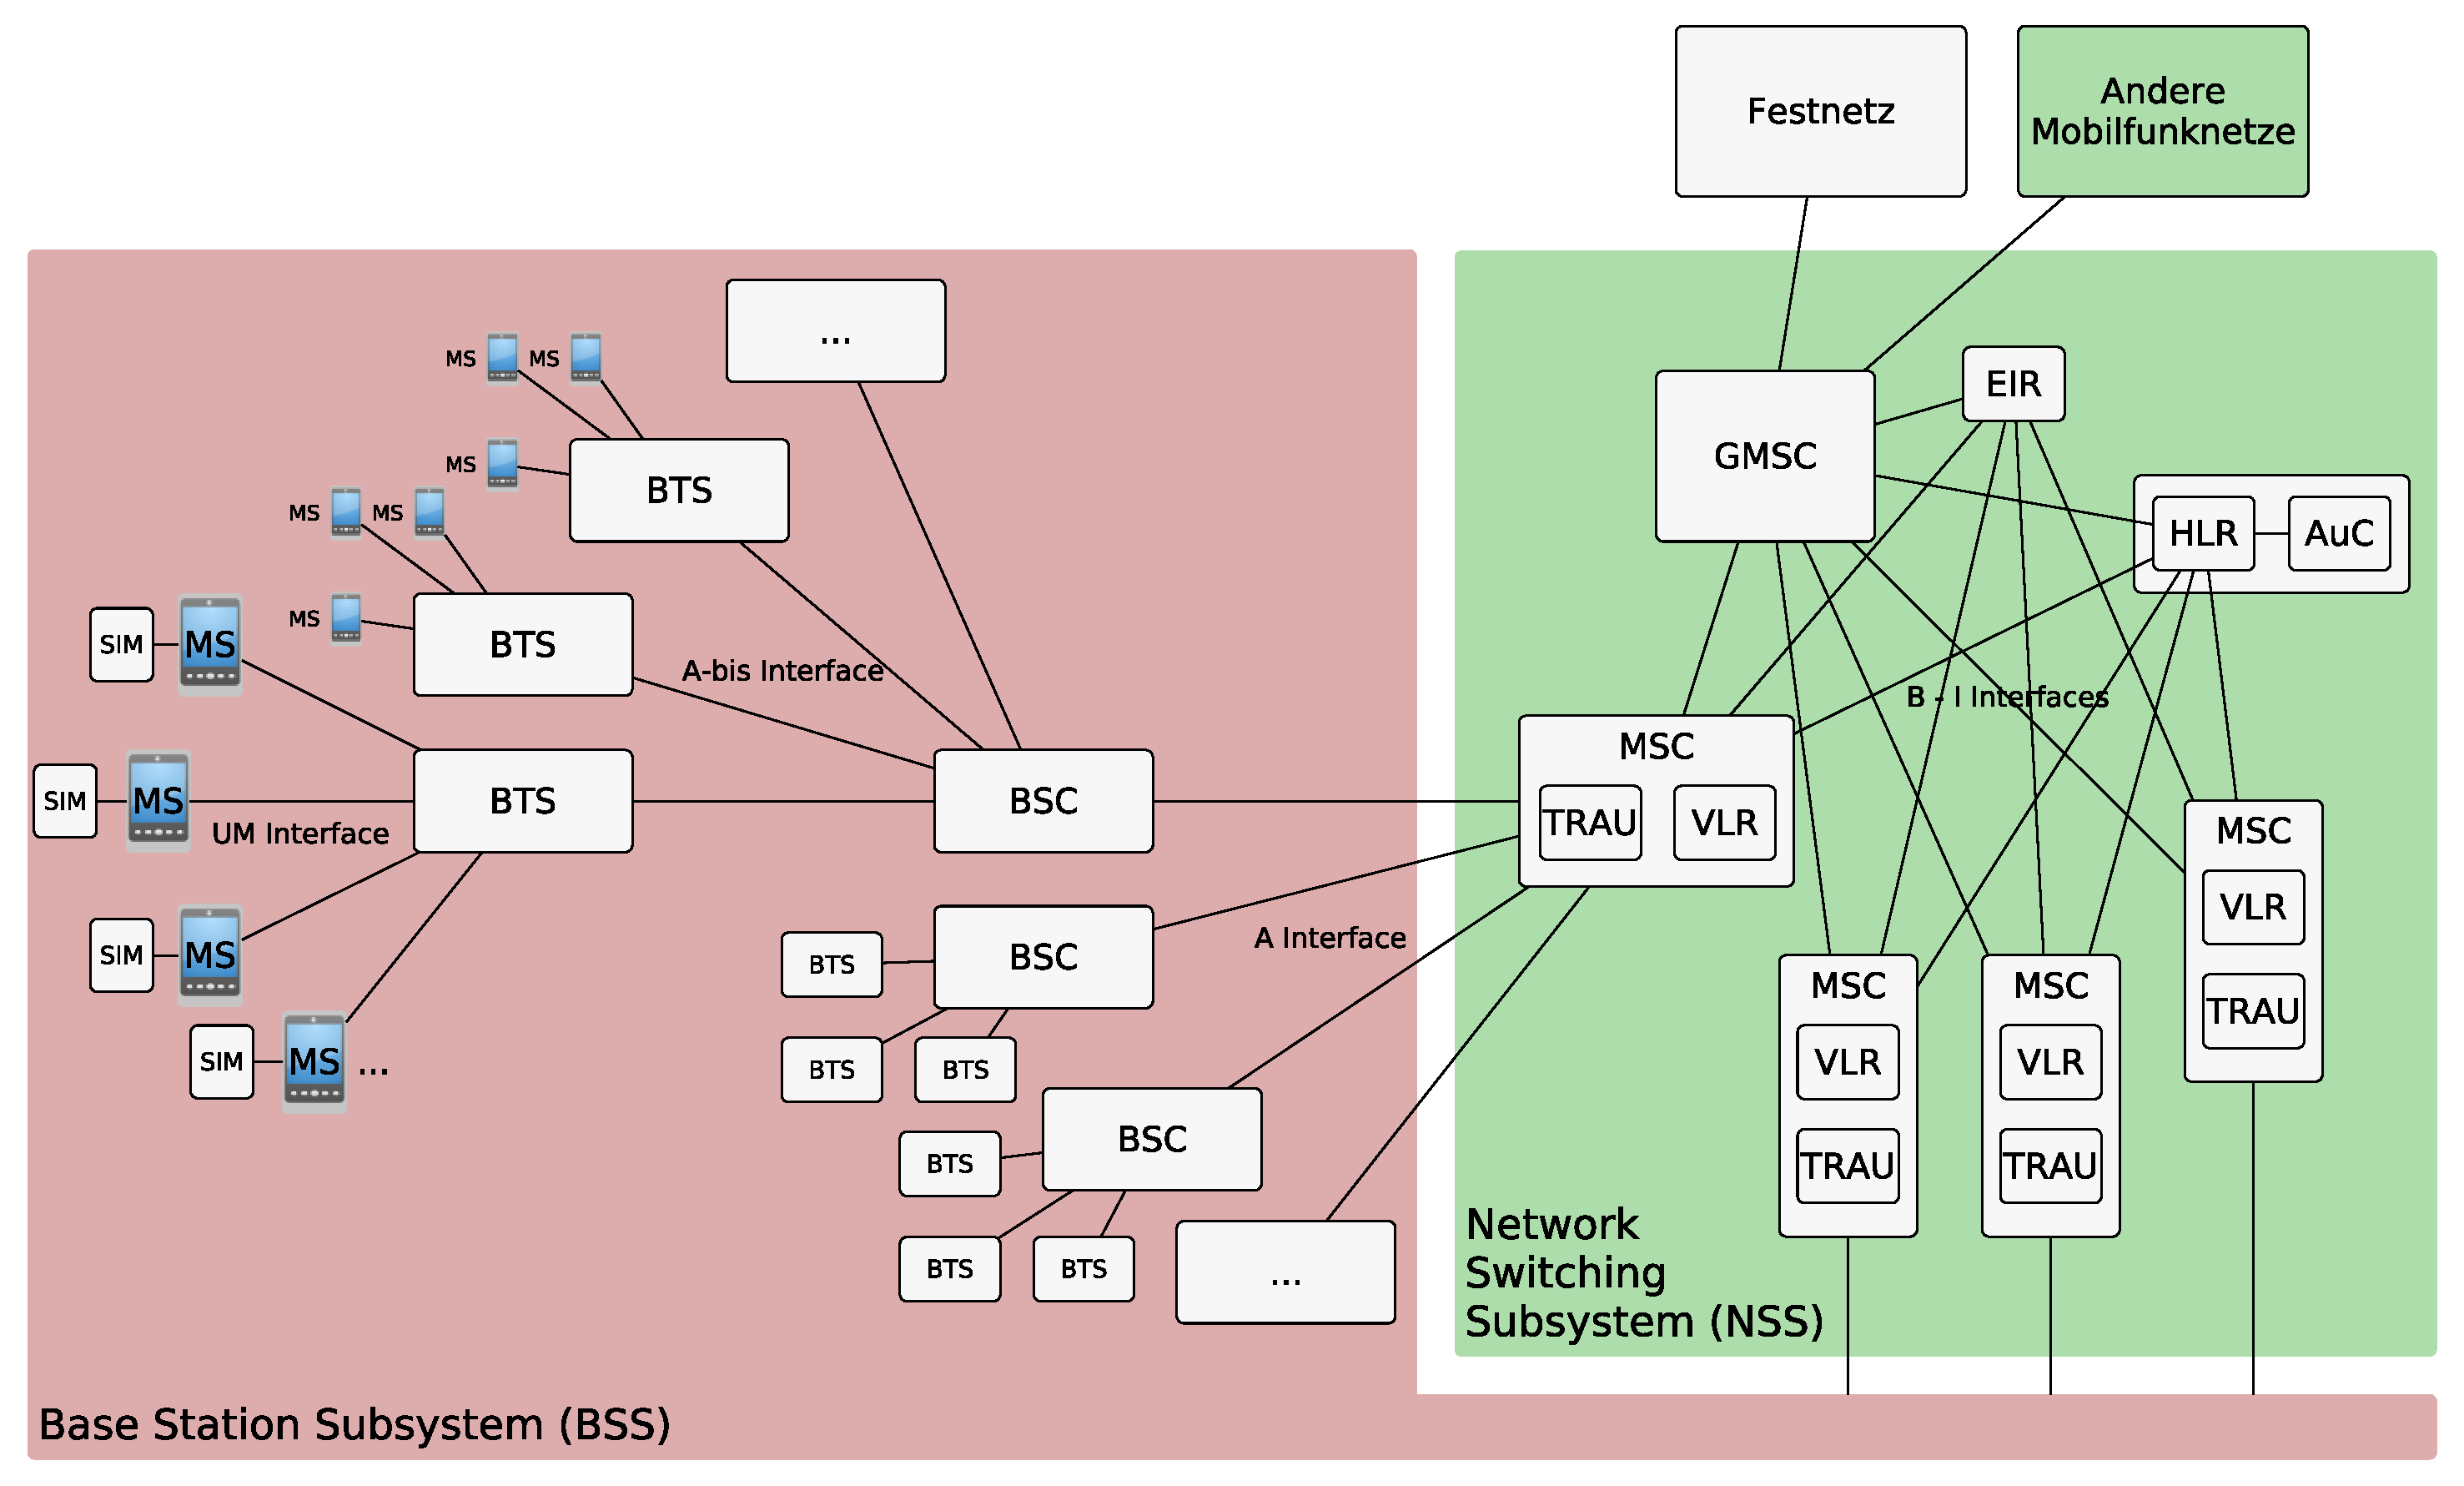
\includegraphics[width=1.0\linewidth]{figures/gsm_network_architecture.pdf}
\end{figure}

\begin{description}
\item[\acused{TRAU}\acs{TRAU} - \acl{TRAU}] Die \ac{TRAU} transkodiert \ac{GSM}-kodierte Sprachdaten in das im Netzwerk verwendete \ac{ISDN} Format (ITU-T A-law). Obwohl sie funktionell dem \ac{BSS} zugeordnet ist, kann sie entweder zwischen \ac{BTS} und \ac{BSC}, oder zwischen \ac{BSC} und \ac{MSC} eingebaut werden. Meist wird sie direkt im \ac{MSC} integriert, da dann weniger \ac{TRAU} Einheiten benötigt werden und Bandbreite auf dem Abis und A Interface gespart wird. \ac{GSM} kodierte Sprachdaten brauchen 13kBit/s, \ac{ISDN} kodierte 64kBit/s. \citep[Kap. 5.2.1]{eberspacher:2008:gsm-architecture}
\item[\acused{EIR}\acs{EIR} - \acl{EIR}] Das \ac{EIR} ist eine optionale Datenbank, die für die Verwaltung von Teilnehmer- und Gerätenummern zuständig ist. Hier werden die \acp{IMEI} von Geräten, die als gestohlen gemeldet wurden, auf einer Blacklist geführt. Diesen kann dann ein Zugriff zum Netz verwehrt werden.
\item[\acused{GMSC}\acs{GMSC} - \acl{GMSC}] Das \ac{GMSC} verbindet mehrere \acp{MSC} mit anderen Mobilfunknetzen und dem Festnetz. Es ist zuständig für die Vermittlung von Anrufen und Nachrichten zwischen diesen. Für Routing zwischen den \acp{PLMN} hat es innerhalb des \ac{SS7} Zugriff auf das \ac{HLR} und \ac{EIR}. In der Regel wird ein reguläres \ac{MSC} zusätzlich an andere \acp{PLMN} angebunden und um die Gateway Funktionalität erweitert.
\item[Abis Schnittstelle]
Die Abis Schnittstelle verbindet \ac{BTS} und \ac{BSC} über E-1 Leitungen. Neben der Weiterleitung von Anwenderdaten erlaubt sie über entsprechende Protokolle die Konfiguration des Transceivers sowie Allokation von Frequenzen im \ac{BTS}.
\item[A Schnittstelle] Das A Interface dient dem Datenaustausch zwischen \ac{BTS} und \ac{MSC}. Letzteres kann darüber Konfigurationsnachrichten an das \ac{BSS} schicken und Nutzerdaten weiterleiten.
\item[B-I Schnittstellen]
Hierbei handelt es sich um Interfaces, die zur Kommunikation zwischen Komponenten des \ac{NSS} definiert wurden. Die Komponenten sind über ein \ac{SS7}-Netzwerk miteinander verbunden und kommunizieren über verschiedene \ac{MAP} Protokolle.
\end{description}

\section{GSM Protokolle und Schnittstellen} \label{hdl:a_schnittstellen_protokolle}

\begin{figure}[H]
  \begin{center}
    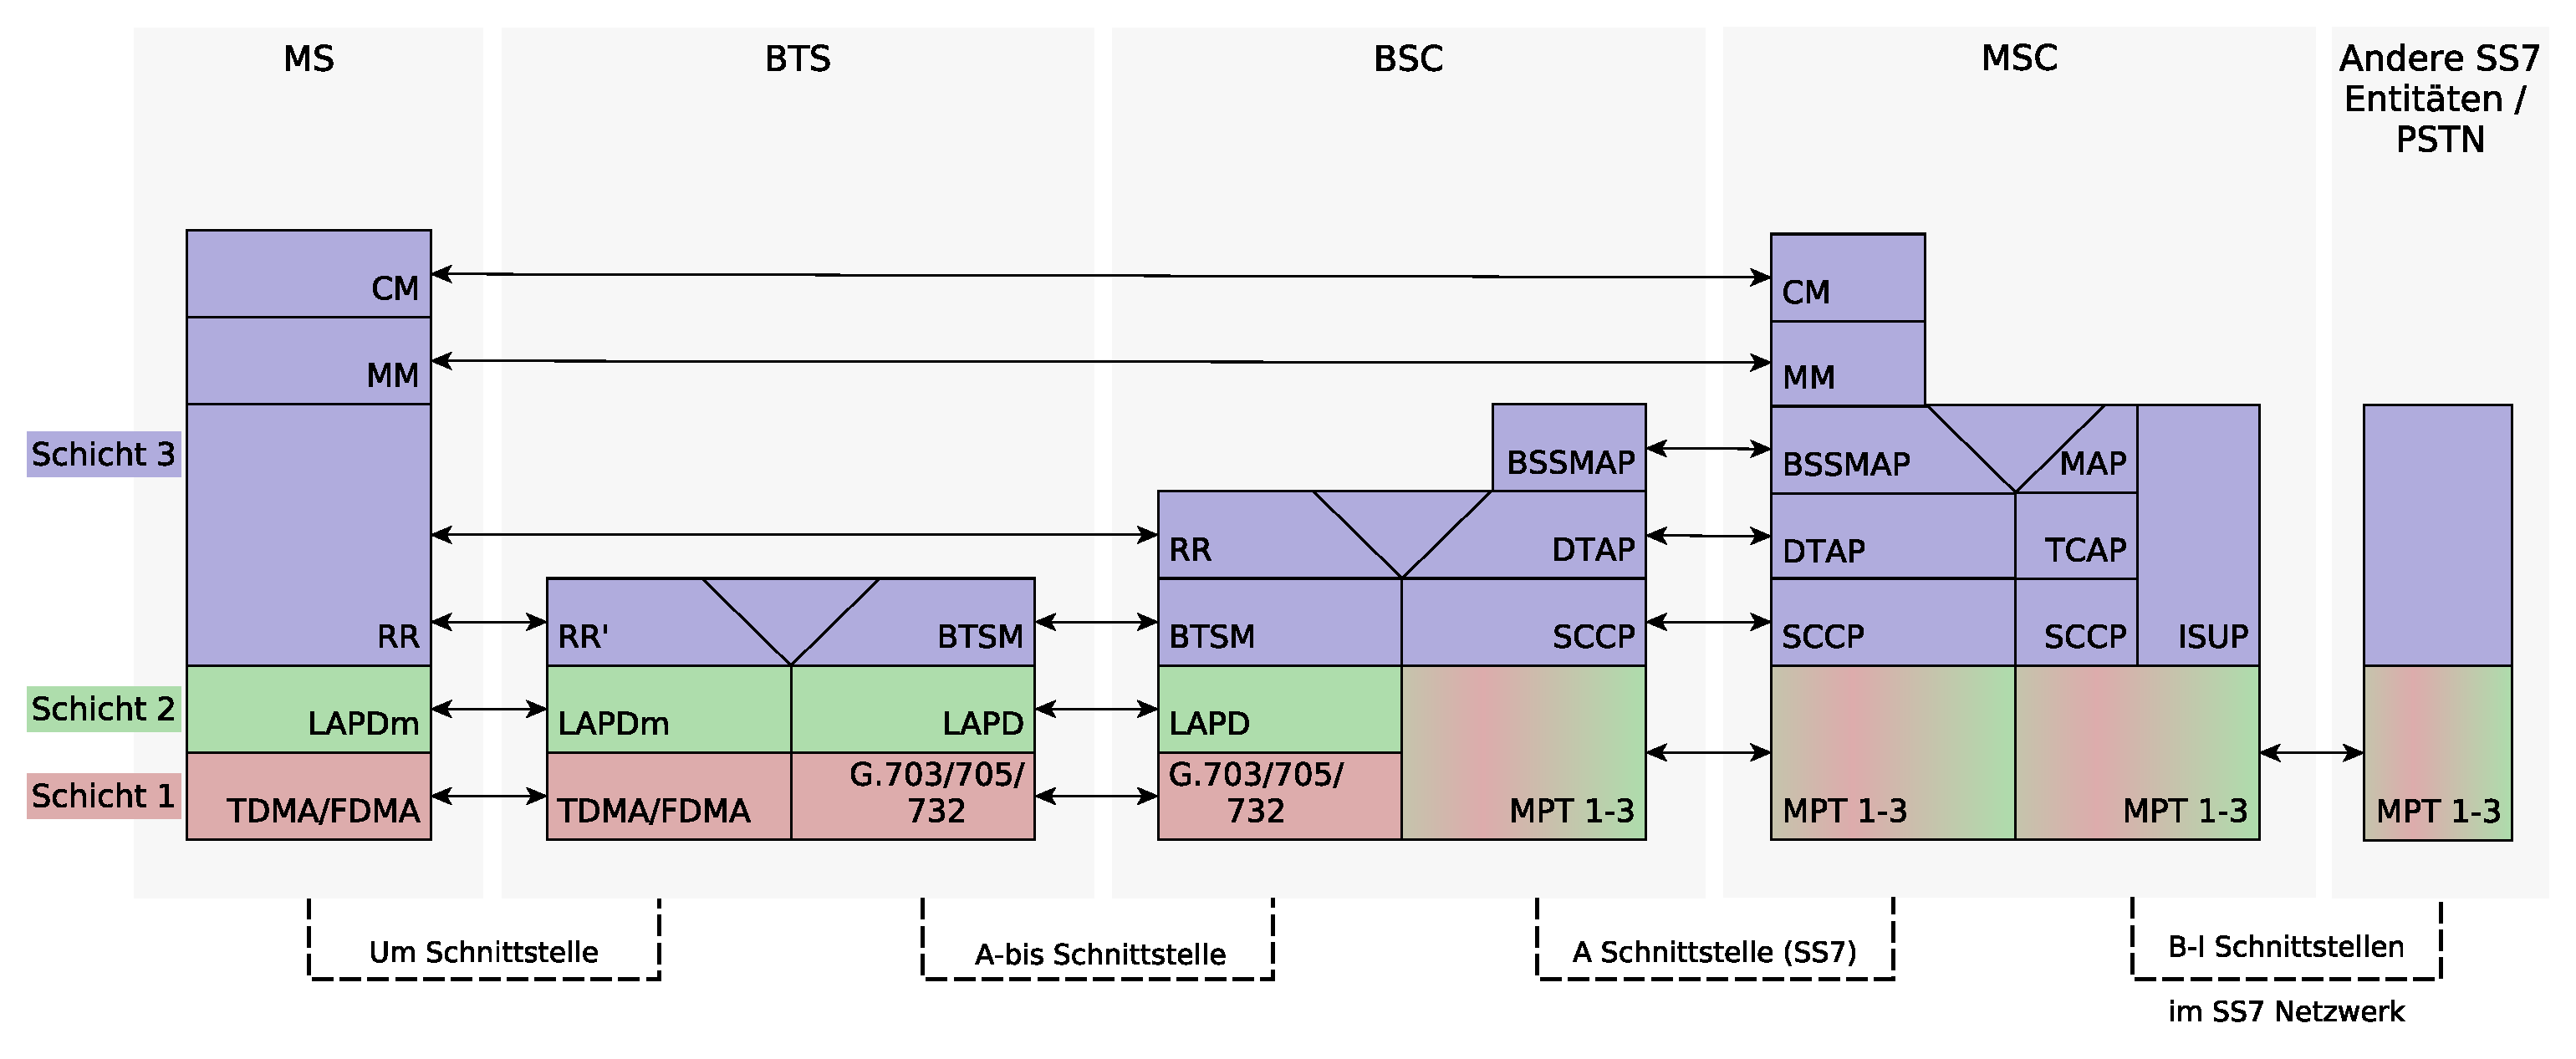
\includegraphics[width=1.0\textwidth]{figures/gsm_protocol_stack.pdf}
  \end{center}
\end{figure}

\subsection{TDMA/FDMA} \label{hdl:a_tdma_fdma}

\ac{GSM} verwendet als Phasenmodulation \ac{GMSK}, um das Spektrum bei Modulation eines digitalen Signals effektiv auszunutzen \citepauthor{3gpp:05.04}. Dadurch kann das in \ac{GSM}-900 zur Verfügung stehende Frequenzband, von 890.0-915.0 MHz für Uplink und 935.0-960.0 MHz für Downlink, in jeweils 124 Trägerfrequenzen mit 200kHz Abstand eingeteilt werden. Über die \acp{ARFCN} werden einer \ac{BTS} Funkkanäle für Uplink und Downlink zugeordnet. \citep{schnabel2003kommunikationstechnik}

In \citetauthor[Kap. 4.3]{3gpp:05.02} wird das in \ac{GSM} verwendete \ac{TDMA} Verfahren spezifiziert. Ein \ac{TDMA} Frame (4.615 ms) besteht darin aus 8 Zeitschlitzen mit einer Zeitdauer von 577 $\mu$s, sogenannten physikalischen Kanälen. Ein mit jedem \ac{TDMA} Frame inkrementierter Zähler gibt an, in welchem Frame man sich gerade befindet.

\begin{figure}[H]
  \begin{center}
    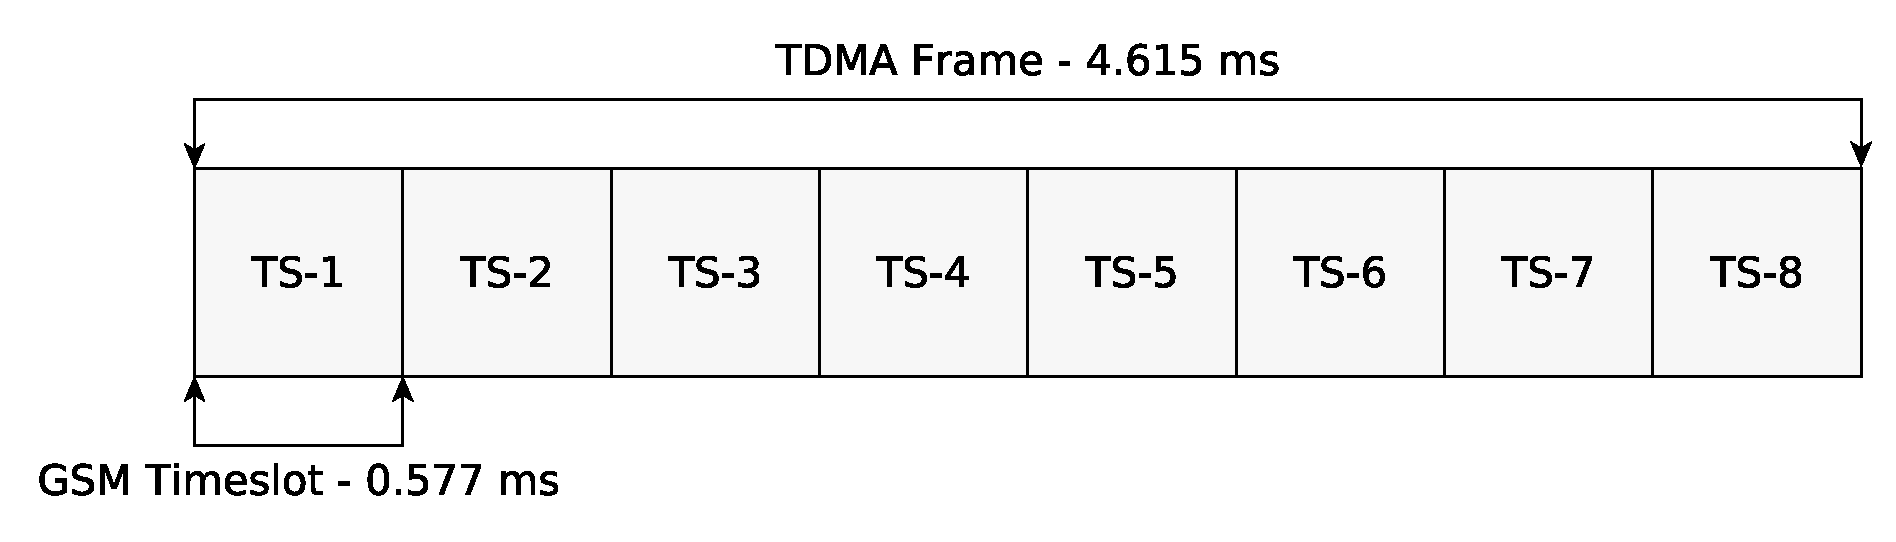
\includegraphics[width=1.0\textwidth]{figures/gsm_timeslots.pdf}
  \end{center}
  \caption[TDMA-Zeitschlitze in GSM]{\ac{TDMA}-Zeitschlitze in \ac{GSM}, nach \citepauthor[Kap. 4.3]{3gpp:05.02}} \label{fig:gsm-timeslots} 
\end{figure}

In einem Timeslot kann die Datenmenge von genau einem \ac{GSM}-Burst übertragen werden. Je nach Inhalt gibt es verschiedene Typen von Bursts, die in \citetauthor[5.2]{3gpp:05.02} nachgelesen werden können. Der Aufbau eines \acp{NB} ist in \autoref{fig:normal_burst} dargestellt. Neben kodierten Daten enthalten Bursts auch eine "`Guard Period"' am Ende, die keine Information mehr enthält, als Puffer zwischen den Timeslots.

Der Uplink wird um 3 Zeitschlitze verzögert mit dem Downlink synchronisiert, damit die \acp{MS} genug Zeit haben auf empfangene Daten zu reagieren. Physikalische Kanäle können unterschiedliche Aufgaben wie Broadcasting (\ac{BCCH}), Signalisierung (\ac{CCCH}) und Sprachdatenübertragung (\ac{TCH}) zugewiesen werden. Durch die Konfiguration von bis zu 7 Sprachkanälen pro Trägerfrequenz können je Trägerfrequenz mehrere Sprachverbindungen gleichzeitig übertragen werden. \citep{schnabel2003kommunikationstechnik}

In der Regel wird TS-0 eine Kombination aus \ac{BCCH} und \ac{CCCH}, TS-1 \ac{CCCH} zugeordnet und die restlichen Kanäle für Sprach- oder Datenübertragung verwendet.

\subsection{Abis Interface} \label{hdl:a_abis}

Die \ac{BSS}-interne Schnittstelle zwischen \ac{BTS} und \ac{BSC} ist nicht standardisiert. Das Abis Interface ermöglicht die Steuerung und Konfiguration der \ac{BTS} über \ac{BTSM} und die Weiterleitung transparenter \ac{RR}, \ac{MM} und \ac{CM} Nachrichten.

Die physikalische Schicht besteht meist aus einer kabelgebundenen Verbindung nach \citetauthor{itu:g.703} (oder 705 / 732) mit 2,048 MBit/s (Europa) oder 1,544 MB/s (USA). Die Bandbreite wird über \ac{TDMA} in 30 Zeitschlitze für Sprache und Daten und zwei Zeitschlitze für Synchronisation und Signalisierung unterteilt.

Für die Datensicherungsschicht wird das \ac{ISDN} Protokoll \ac{LAPD} verwendet. Dessen Aufgabe ist der zuverlässige Datentransfer zwischen \ac{BTS} und \ac{BSC} auf dem D-Kanal. Der D-Kanal ist in \ac{ISDN} der Kanal zur Übertragung von Steuerinformationen. Für \ac{ISDN} ist das Protokoll in \citetauthor{itu:q.920} und \citetauthor{itu:q.921} spezifiziert, die \ac{GSM} Adaption findet man in \citetauthor{3gpp:08.56}.

\ac{LAPD} umfasst folgende allgemeine Funktionen:
\begin{itemize}
\item Bereitstellung von einem oder mehreren \ac{LAPD}-Verbindungen auf dem D-Kanal
\item Bereitstellung einer zuverlässigen Verbindung auf dem D-Kanal
\item Ablaufkontrolle
\item Flußkontrolle
\item Fehlererkennung und Korrekturmechanismen
\item Benachrichtigung von Layer 3 Einheiten bei fatalen Fehlern
\end{itemize}

Für Layer 3 werden mehrere \ac{LAPD}-Verbindungen zur Verfügung gestellt, die über verschiedene \acp{SAPI} unterschieden werden. Jede \ac{SAPI} verwendet dabei ein eigenes Protokoll. Layer 3 auf der A-bis Schnittstelle ist in \citetauthor{3gpp:08.58} beschrieben.

Übersicht über die Protokolle der \acp{SAPI}:
\begin{description}
\item [SAPI 0, \acf{RSL}] wird für Weiterleitung des Datenverkehrs von und an die Luftschnittstelle verwendet, also \ac{RR}-Signalisierungsnachrichten und die transparenten \ac{CC} und \ac{CM} Nachrichten.
\item [SAPI 62, \acf{OML}] wird für Verwaltung, Konfiguration und Überwachung des \ac{BTS} und seiner Transceivereinheiten verwendet.
\item [SAPI 63, \acf{L2ML}] ist für die dynamische Verwaltung von \acp{TEI} und der Adressierung der Transceivern zuständig.
\end{description}

\subsection{A Interface} \label{hdl:a_a_interface}

Das A Interface liegt zwischen \ac{BSC} und \ac{MSC}. Der Protokollstack basiert auf dem \ac{SS7} Standard, der auch für die Signalisierung im restlichen \ac{NSS} verwendet wird. Die physikalische Verbindung ist, wie beim Abis Interface, kabelgebunden mit 2,048 oder 1,544 MBit/s. Sie wird über \ac{TDMA} in 32 Kanäle unterteilt. Davon werden 30 für Datenübertragung und zwei für Signalisierung verwendet. Bei Positionierung der \ac{TRAU} im \ac{BSC} \ac{TRAU} benötigt ein Sprachkanal im \ac{ISDN} Format 64 kBit/s und füllt damit einen kompletten Slot aus. Es können also bis zu 30 Verbindungen gleichzeitig unterstützt werden. Sitzt die \ac{TRAU} hingegen im \ac{MSC}, braucht ein Sprachkanal nur 16 kBit/s. Dadurch sind mehr gleichzeitige Verbindungen möglich. 

Schicht 1 und 2 verwenden in \ac{SS7} definierte \ac{MTP}, die eine zuverlässige Verbindung zwischen \ac{BSC} und \ac{MSC} gewährleisten.

\ac{SCCP} ermöglicht auf Schicht 3 eine globale Adressierung von Elementen im \ac{SS7}-Netzwerk. Mit \ac{BSSMAP} Nachrichten kann das \ac{BSS} vom \ac{MSC} konfiguriert und überwacht werden. Des Weiteren stellt \ac{SCCP} verbindungslose und verbindungsorientierte Nachrichtenflüsse für \acf{RR}, \ac{CM} und \ac{MM} zur Verfügung.

\section{A5 Verschlüsselungsverfahren}\label{hdl:a_a5}
Von \ac{3GPP} aktuell (Stand 2017) spezifizierte, synchrone Verschlüsselungsverfahren auf der Funkschnittstelle.

\subsection{A5/0}
Wird A5/0 ausgehandelt, ist die Verbindung auf der Luftschnittstelle unverschlüsselt. In \citetauthor[4.8]{3gpp:03.20} wird zwar ausdrücklich erwähnt, dass Mobiltelefonen die nur A5/0 unterstützen, abgewiesen werden sollen, umgekehrt gilt das aber nicht. So akzeptieren die meisten Handys eine unverschlüsselte Verbindung, wenn die \ac{BTS} diese fordert. Dem Benutzer wird das oft nicht signalisiert. 

A5/0 wird von echten \ac{BTS} der Netzbetreiber nicht verwendet, Angreifer mit falschen \ac{BTS} können diese Schwachstelle aber nutzen.

\subsection{A5/1}

A5/1 ist eine 1987 für \ac{GSM} entwickelte Stromchiffre und war bis zur Veröffentlichung von A5/3 der sicherste verfügbare Algorithmus.

Die geringe Schlüsselänge von 64 Bit in Kombination mit Schwachstellen gegen Angriffe mit bekanntem Klartext macht den Algorithmus verwundbar \citep{golic1997cryptanalysis}. \citet{nohl2010wideband} führte auf der 27C3 vor, dass eine A5/1 verschlüsselte Verbindung mit handelsüblicher und kostengünstiger Hardware in Echtzeit gebrochen werden kann. Da die für den Angriff verwendeten Rainbow Tables veröffentlicht wurden, kann der Angriff seitdem mit geringem eigenen Aufwand von beliebigen Angreifern ausgeführt werden.

A5/1 wird trotz seiner Schwächen auch 2017 noch mit einem Anteil von ca. 50\% im \ac{GSM}-Netz verwendet \citep{gsmmap:secrep-ger}. 

\subsection{A5/2}

A5/2 ist eine Stromchiffre, die 1989 für Exportländer von \ac{GSM} entwickelt wurde. Mit nur 50 Bit Entropie im kryptografischen Schlüssel ist der Algorithmus deutlich schwächer als A5/1 und wurde von \citet{barkan2003instant} in Echtzeit geknackt.

Um 2007 wurde in den \ac{3GPP} Meetings festgelegt, dass A5/2 offiziell nicht mehr von neuen Mobiltelefonen und im \ac{GSM}-Netz unterstützt werden soll. Alle Netzbetreiber davon zu überzeugen sollte aber noch bis 2008 dauern. \citep{osmocom:withdrawal-a52}

\subsection{A5/3, GEA3}

Der A5/3 Algorithmus basiert auf der Blockchiffre KASUMI \citepauthor{3gpp:35.202} und wurde 2002 in \citetauthor{3gpp:55.216} im Zuge der \ac{EDGE}/\ac{EGPRS} Entwicklung als Nachfolger von A5/1 spezifiziert. In \ac{UMTS} wird der Algorithmus standardmäßig unterstützt, in \ac{GSM} musste er von den Netzbetreibern erst nachgerüstet werden, was den Einzug in \ac{GSM}-Netzwerken hinauszögerte. In Deutschland wurde A5/3 erst 2013 von der Deutschen Telekom zusätzlich zu A5/1 für \ac{GSM} eingeführt \citep{telekom:a53-gsm}.

\autoref{fig:fig-a53-encryption} veranschaulicht das Mapping der Input- und Outputparameter auf die KASUMI-KGCORE-Funktion. Dabei ist \ac{Kc} der vom \ac{A8} aus dem geheimen Schlüssel des Mobilfunkteilnehmers generierte Schlüssel und COUNT die Framenumber der zu verschlüsselnden Nachricht. Die Framenumber kann den maximalen Wert von 2715648 erreichen, wofür die 22 verwendeten Bits ausreichen. A5/3 verwendet KASUMI nur mit 64 Bit Entropie, der von KASUMI verlangte Schlüsselparameter mit 128 Bit wird durch Konkatenation von zwei 64 Bit Schlüsseln erreicht.

Als Ergebnis liefert die Funktion zwei Blöcke BLOCK1 und BLOCK2 mit 114 Bits, die für die Verschlüsselung und Entschlüsselung von je einem Uplink und Downlink Burst verwendet werden. Verschlüsselt wird über binäre Addition der Datenbits mit dem Schlüsselstrom.

\begin{figure}[H]
  \begin{center}
    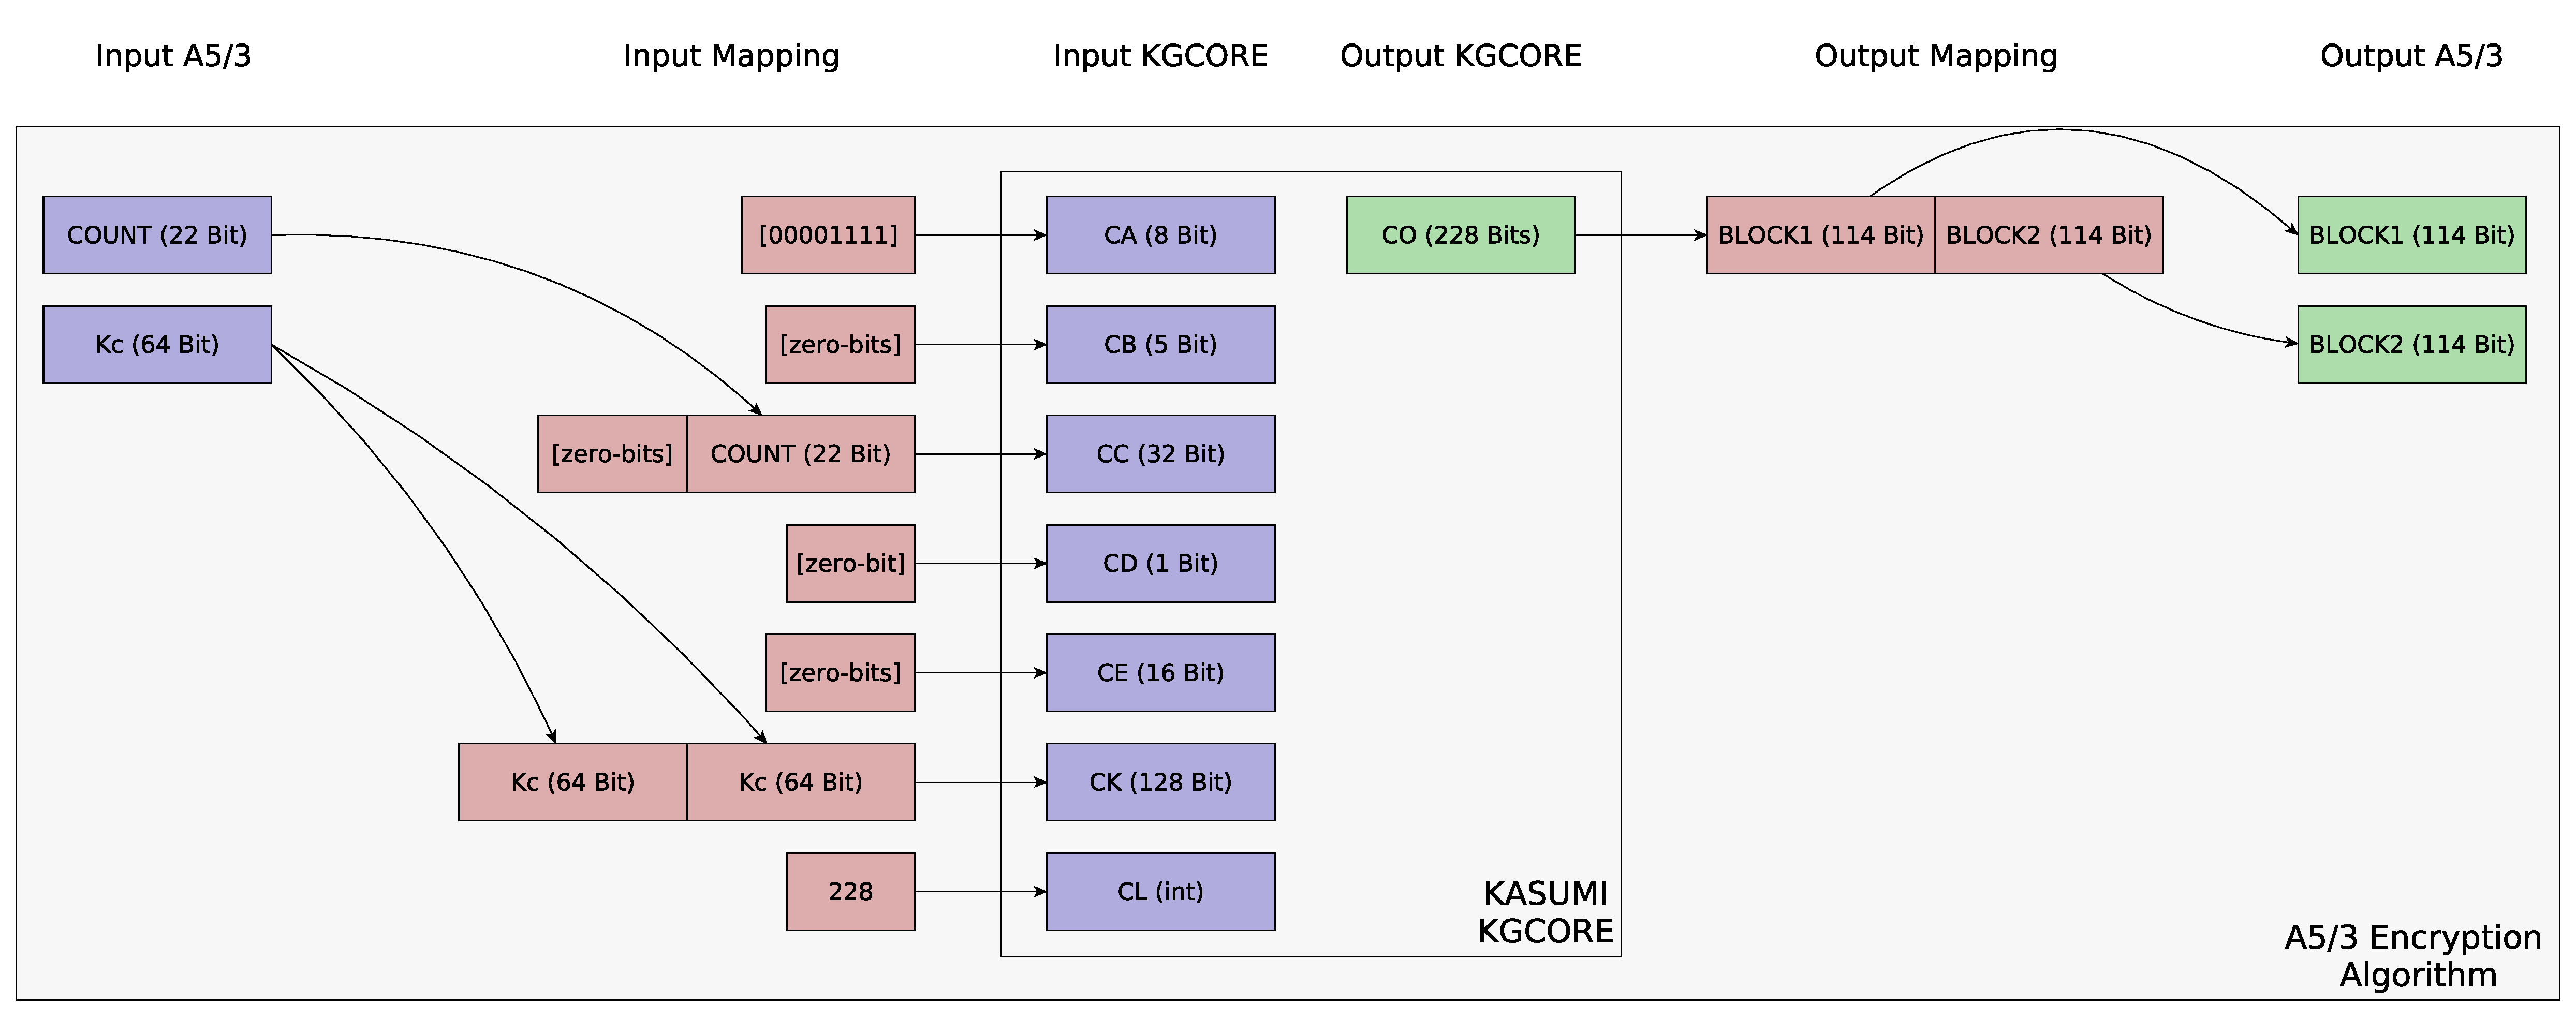
\includegraphics[width=1.0\textwidth]{figures/a53_encryption.pdf}
  \end{center}
  \caption[Das Parameter Mapping von A5/3 auf die Kasumi-KGCORE-Funktion]{Das Parameter Mapping von A5/3 auf die Kasumi-KGCORE-Funktion, erstellt mit yEd} \label{fig:fig-a53-encryption}
\end{figure}

Kasumi konnte von \citet{dunkelman2010practical} geknackt werden. Allerdings kann der Angriff nicht auf seine Verwendung im A5/3 Algorithmus angewendet werden. Trotz seiner geringen effektiven Schlüssellänge von 64 Bit gilt er deshalb als relativ sicher. Die Schlüssellänge macht ihn jedoch grundsätzlich verwundbar für Bruteforce Attacken. \citep{nohl2014mobile}

A5/3 ist der sicherste aktuell in \ac{GSM}-Netzwerken verwendete Algorithmus und deshalb für den vorgestellten Angriff von besonderem Interesse.

\subsection{A5/4, GEA4}
Ein in \citetauthor{3gpp:55.226} spezifiziertes Verschlüsselungsverfahren, das wie A5/3 auf KASUMI basiert, im Gegensatz zu diesem aber die kompletten verfügbaren 128 Bit als Schlüssel verwendet.

Der Algorithmus wird in aktuellen 2G Netzwerken nicht verwendet.

\subsection{GIA5, GEA5}
Ein recht neuer Algorithmus, der 2016 in \citetauthor{3gpp:55.226} spezifiziert wurde.

Der Algorithmus wird in aktuellen 2G Netzwerken nicht verwendet.

\section{Frequency-Hopping}

Frequency-Hopping kann in \ac{GSM} optional verwendet werden, um für die Übertragung von Daten ein breiteres Frequenzspektrum zu benutzen. Dabei springt die Trägerfrequenz innerhalb eines bestimmten Bereichs. Die Sprungparameter werden in einer bestehenden Verbindung vom \ac{BTS} vorgegeben und dem Endgerät im \ac{SDCCH} mitgeteilt.

Damit werden auf der Luftschnittstelle häufige frequenzbedingte Übertragungsprobleme verringert und das Signal-Rausch-Verhältnis verbessert. Frequency Hopping ist - solange eine nicht vorhersehbare Hopping Sequenz verwendet wird - auch eine sicherheitsrelevante Funktion. Die Zuweisung von abgefangenen Signalen zu einer Verbindung wird ohne das Wissen der verwendeten Sprungsequenz erschwert.

\ac{GSM} definiert in \citetauthor{3gpp:05.02} folgende Parameter für Frequency Hopping:
\begin{description}
\item[\acf{MA}] Eine Liste von erlaubten Sprungfrequenzen für das Mobiltelefon. Es können maximal 63 Frequenzen angegeben werden.
\item[\acf{HSN}] Legt die in der Zelle verwendete Sprungsequenz fest. Es können 64 verschiedene \acp{HSN} verwendet werden. \ac{HSN} = 0 bedeutet zyklisches Springen, die Werte 1 bis 63 geben verschiedene pseudo-zufällige Sequenzen vor.
\item[\acf{MAIO}] Legt die Startfrequenz fest, auf der die \ac{MS} zu Senden beginnt. Der Wert kann zwischen 0 und der maximal in \ac{MA} festgelegten Anzahl an unterstützten Frequenzen liegen.
\end{description}